% -*- root: 00-main.tex -*-
\section{Results}
\label{sec:results}

\subsection{Proof of concept on digital phantoms}
\label{sec:results_phantom}
Using a simplified subset of the experimental instrumentation described in
  \autoref{sec:experiments_evaluation}, we collected quantitative results on the digital
  phantoms.
A total of 1200 registration experiments (4 phantom types $\times$ 150 random warpings
  $\times$ 2 resolutions) were run.
Parameter settings of every processing step in the experiments are made available along with
  the source code.
For each registration, the averaged Hausdorff distance (see \autoref{sec:experiments_evaluation})
  of the inner and the outer surfaces was computed.
The results showed a consistent and high accuracy, below the image resolution.
\autoref{fig:phantom} (block C) presents the violin plots by model type corresponding
  to the two sets of resolutions of generated phantoms.
To support that the misregistration errors averaged per experiment was significantly
  under the resolution of the target image, we proceeded as follows.
First, we confirmed that the error distributions were skewed using a Shapiro-Wilk test of
  normality.
All the distributions of errors under test (4 phantom types $\times$ 2 resolutions) resulted
  non-normal with $p<0.001$.
Consequently, we used the non-parametric Wilcoxon signed-rank test along with Bonferroni
  correction for multiple comparisons ($N=150$).
Averaged errors resulted significantly lower than voxel size with $p < (0.001 / 150)$
  for all the tests (4 phantom types $\times$ 2 resolutions).
Since statistical tests may not be conclusive enough, we also computed the confidence intervals
  (\autoref{tab:ci_phantom}).


\begin{table}
		\centering
		\footnotesize
    \begin{tabular}{lccccc}
    Res. & ``gyrus'' & ``ball''  & ``box''   & ``L''     & Aggreg.    \\\hline
    Low  & 0.59-0.60 & 0.65-0.76 & 0.68-0.71 & 0.67-0.77 & 0.64-0.66  \\
    High & 0.18-0.38 & 0.31-0.45 & 0.34-0.42 & 0.34-0.40 & 0.34-0.38  \\
    \hline
    \end{tabular}
    \caption{95\% Confidence Intervals (CIs) were computed using bootstrapping of $10^4$ samples,
      for each phantom type and resolution.
    Taking into account the non-normal distribution of errors, we used the median as location
  		statistic.
    All the CIs were below the corresponding half-voxel size in all the phantom types.}\label{tab:ci_phantom}
\end{table}

\subsection{Correction of distortions on real datasets}\label{sec:results_hcp}

\paragraph*{Assessing the segmentation model}\label{sec:res_model_and_metric} %
%
Preliminarily, we investigated the aptness of our segmentation model to play as cost function
  driving the registration process.
First, we evaluated several alternative models to segment the target bivariate images
  (\gls*{fa} and \gls*{adc}).
Based on the observed joint distribution of each (\suppl{section S4}),
  we selected the 6-regions scheme described in \autoref{sec:human_connectome}.

The distortions follow expression \eqref{eq:fieldmap} and hence, we easily reduced the
  error space to one dimension as follows.
The energy functional \eqref{eq:energy} was evaluated for the warpings given by
  a linearized space of distortions
  $\hat{U} = \epsilon \cdot U_{true} = \vec{r} + \epsilon \cdot u(\vec{r})$,
  with $\epsilon \in [-1.1, 1.1]$.
The results of this experiment are shown in \autoref{fig:energymap}.
The metric consistently displayed its minimum at $\epsilon=0.0$ (ground-truth location).

\begin{figure}
	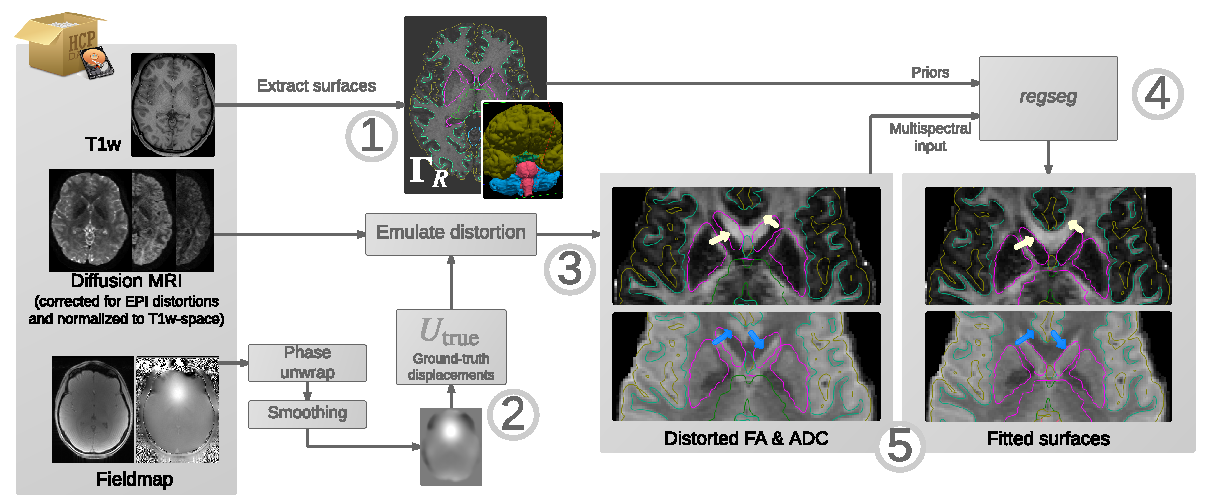
\includegraphics[width=\linewidth]{figures/figure04.pdf}
	\caption{Assessment of the segmentation model, sampling the value of the energy functional
	\eqref{eq:energy} versus several registration errors generated as explained in
	\autoref{sec:res_model_and_metric}.
	The metric of our registration method displayed a smooth gradient towards the minimum
	located at the $\epsilon = 0.0$ point.}\label{fig:energymap}
\end{figure}

\paragraph*{Evaluation \& cross-comparison}\label{sec:res_cc_evaluation}
%
Finally, we compared the performance of \emph{regseg} and the standard \gls*{t2b}
  correction.
We computed the \gls*{swindex} \eqref{eq:swindex} of every surface after correction,
  for both \emph{regseg} and the \gls*{t2b} methods.
Finally, to statistically compare the results, we performed a one-way ANOVA test
  on the warping indices for three specific surfaces of interest
  ($\Gamma_{VdGM}$, $\Gamma_{WM}$, and $\Gamma_{pial}$).
These interfaces are critical in analyses of whole-brain tractography.
The one-way ANOVA evidenced that error distributions were significantly different,
  $p \approx 2 \times 10^{-9}$.
We also reported the 95\% CIs of the \gls*{swindex} for those surfaces.
The aggregated CI for \emph{regseg} was $[1.08 - 1.50] mm$, whereas the competing method
  yielded an aggregated CI of $[2.06 - 2.43] mm$.
The quantitative results of the ANOVA tests and the CIs are presented in \autoref{tab:results_real}.
Visual assessment of one case is shown in \autoref{fig:results_real}, along with the corresponding
  violin plots of error distributions by correction method and surface.
Extended visual assessment of the 16 cases is included in the \suppl{section S5}.

\begin{table}
		\centering
		\footnotesize
		\tabcolsep=0.05cm
    \begin{tabular}{cccccc}
    & & $\Gamma_{VdGM}$  & $\Gamma_{WM}$ & $\Gamma_{pial}$ & Aggregated \\
    \hline
    \multirow{2}{*}{CI}
       & \emph{regseg}        & 0.77 - 1.18 & 0.95 - 1.85 & 1.33 - 2.13 & 1.08 - 1.50 \\
       & T2B                  & 1.73 - 2.62 & 1.96 - 2.40 & 2.16 - 2.63 & 2.06 - 2.43 \\
    \hline
    \multirow{2}{*}{ANOVA}
       & p-value  & 1.4$\times$10$^{-5}$& 1.3$\times$10$^{-3}$& 2.5$\times$10$^{-3}$ & 2$\times$10$^{-9}$ \\
       & f-stat   & 27.87               & 12.89               & 11.13                & 45.04 \\
    \hline
    \end{tabular}
    \caption{All the 95\% CIs of the \gls*{swindex} distributions computed for the
      surfaces of interest were lower for \emph{regseg} with respect to the competing
      method.
    CIs reported in this table were computed using bootstrapping with mean as location
      statistic and $10^4$ samples.
    One-way-ANOVA tests indicated that there is a significant difference between our method and
      the competing method of choice.
    }\label{tab:results_real}
\end{table}

\begin{figure*}
    \centering
    \resizebox{\textwidth}{!}{%
      \begin{tikzpicture}
        \node[inner sep=15pt, draw=black!40](fig05a) at (0,11)
          {\hspace*{20pt}\includegraphics[width=\linewidth]{figures/figure05-a}};
        \node[inner sep=15pt, draw=black!40](fig05b) at (0,0)
          {\hspace*{20pt}\includegraphics[width=\linewidth]{figures/figure05-b}};
        % \node[inner sep=5pt, draw=black!40](fig03c) at (0,0)
        %   {\includegraphics[width=\linewidth]{figures/figure03-c}};
        \node[circle, text=black!75] at (-9.5,17) {\Huge \textbf{A}};
        \node[circle, text=black!75] at (-9.5,3) {\Huge \textbf{B}};
        % \node[circle, text=black!75] at (-8.8,3.4) {\Huge \textbf{C}};
      \end{tikzpicture}
    }%
	\caption{The evaluation instrument automatically renders the overlay between the
	  target \gls*{fa} image and the resulting contours after distortion estimation (yellow color) and
	  their theoretical location using the ground-truth (green color).
	The first two rows show several axial slices for \emph{regseg} (``proposed'' row) and the
	  competing method.
	The last two rows represent the sagittal view.
	We intentionally omitted the coronal slicing as it is the least informative, given the directional property
	  of distortions.
	Red arrows point to regions where the accuracy of the proposed method more clearly overperformed
	  the competing method.
	}\label{fig:results_real}
\end{figure*}